\section{Accelerating X-Blossom on CPUs and GPUs}
We accelerate the original multi-core CPU implementation of X-Blossom in two steps. 
First, we propose X-Blossom-Pro, an optimized CPU realization that introduces alternating-tree reuse to remove duplicated computation across augmenting-path searches.
% and yields up to $3.26\times$ speedup over the original CPU implementation. 
Second, we develop X-Blossom++, the first GPU implementation of the blossom algorithm.
X-Blossom++ maps X-Blossom-Pro's dynamic data structures to GPUs and uses fine-grained edge-level GPU load balancing.
% As a result, X-Blossom++ achieves up to $39.09\times$ speedup over X-Blossom-Pro.

\subsection{X-Blossom-Pro: An Enhanced Implementation of X-Blossom for Multi-Core CPUs}
\label{subsec:reuse}
Maximum matching invokes augmenting-path search repeatedly.
After a matching augmentation between two calls, the previously exposed roots of alternating trees that participate in a discovered augmenting path become matched.
These newly matched vertices can no longer serve as valid exposed roots, so their associated trees must be cleared.
% Connecting Sentence
Algo.~\ref{Algo:XBlossom} handles this root-status change by clearing all alternating trees before each subsequent call, but this is overly conservative.
Trees not involved in any discovered augmenting path remain rooted at exposed vertices, structurally intact, and reusable across iterations.
% Since their roots remain exposed after augmentation, 

% \vspace{-4pt}
\begin{algorithm}[!htbp]
  % \small
  \footnotesize
  \captionsetup{font = footnotesize}
  \caption{Parallel Augmenting-Path Search Procedure with Reusable Alternating Trees in X-Blossom-Pro}
  \label{Algo:Reuse}
  \begin{algorithmic}[1]

  \Require Graph $G$ and matching $M$
  \Ensure A set of vertex-disjoint augmenting paths $P$, or empty if none exist

  \State $S_{\text{exposed}} \gets $ set of exposed vertices
  \State $S_{\text{reuse}} \gets $ non-root even nodes in surviving alternating trees
  \State $S_{\text{reset}} \gets $ non-root even nodes in cleared alternating trees
  \State $N \gets  S_{\text{exposed}} \cup S_{\text{reuse}} $
  \State $F \gets F_\text{old} \cup S_{\text{exposed}} - S_{\text{reset}}$
 
  \State $P \gets \emptyset$
  
  \While{$P = \emptyset \wedge N \neq \emptyset$}

      \State $P \gets$ \Call{Parallel-Augmenting-Path-Detection}{$G, M, N, F$}
      % \If{$P_{\text{total}} \neq \emptyset$}
      %     \State \Return $P_{\text{total}}$
      % \EndIf

      \State $N_{\text{next1}} \gets$ \Call{Parallel-Expand-Alternating-Trees}{$G, M, N, F$}

      \State $N_{\text{next2}} \gets$ \Call{Parallel-Blossom-Handling}{$G, M, N, F$}
      
      \State $N \gets N_{\text{next1}} \cup N_{\text{next2}}$

  \EndWhile
  
  \State \Return $P$

  \end{algorithmic}
\end{algorithm}

Motivated by alternating-tree reuse in bipartite graphs~\cite{akathoott2025bidirectional}, we extend reuse to general graphs with blossoms.
Algo.~\ref{Algo:Reuse} partitions even vertices after each augmentation into exposed vertices, reusable non-root even vertices in surviving trees, and non-root even vertices in trees that must be reset (lines 1--3).
The new checking set combines exposed and reusable even vertices (line 4), so all retained vertices re-enter the three parallel subroutines and preserve the correctness guarantee of~\cite{fan2025x}.
The alternating forest then keeps only surviving trees and removes those whose roots became matched (line 5).
The remaining search follows Algo.~\ref{Algo:XBlossom} while avoiding regrowth of structurally valid trees.


\subsection{X-Blossom++: The First GPU-Accelerated Blossom Algorithm Implementation}
\label{subsec:xb++}
% In this section, we present the first GPU implementation of the blossom algorithm, termed X-Blossom++. Building upon the optimizations introduced in X-Blossom-Pro, X-Blossom++ maps the algorithm’s dynamic data structures onto GPUs and further addresses the inherent irregular and imbalanced parallelism of X-Blossom.

% This is an easy one, but still worth mentioning as one necessary step. 
\subsubsection{Dynamic Data Structure Representations on GPUs}
\label{subsub:repOnGPU}
% Introduction to GPU representation of path tables
X-Blossom uses highly dynamic structures, including the path table and checking set, with frequent insertions and deletions.
On CPUs, standard resizable containers handle allocation, growth, and reclamation efficiently.
On GPUs, CUDA allocation APIs such as \texttt{cudaMalloc} and \texttt{cudaFree} are costly~\cite{guo2024gmlake}, and higher-level containers such as Thrust inherit this cost under frequent updates.
Thus, X-Blossom++ uses explicit memory-management strategies for these dynamic structures.

\begin{figure}[!h]
	\centering
	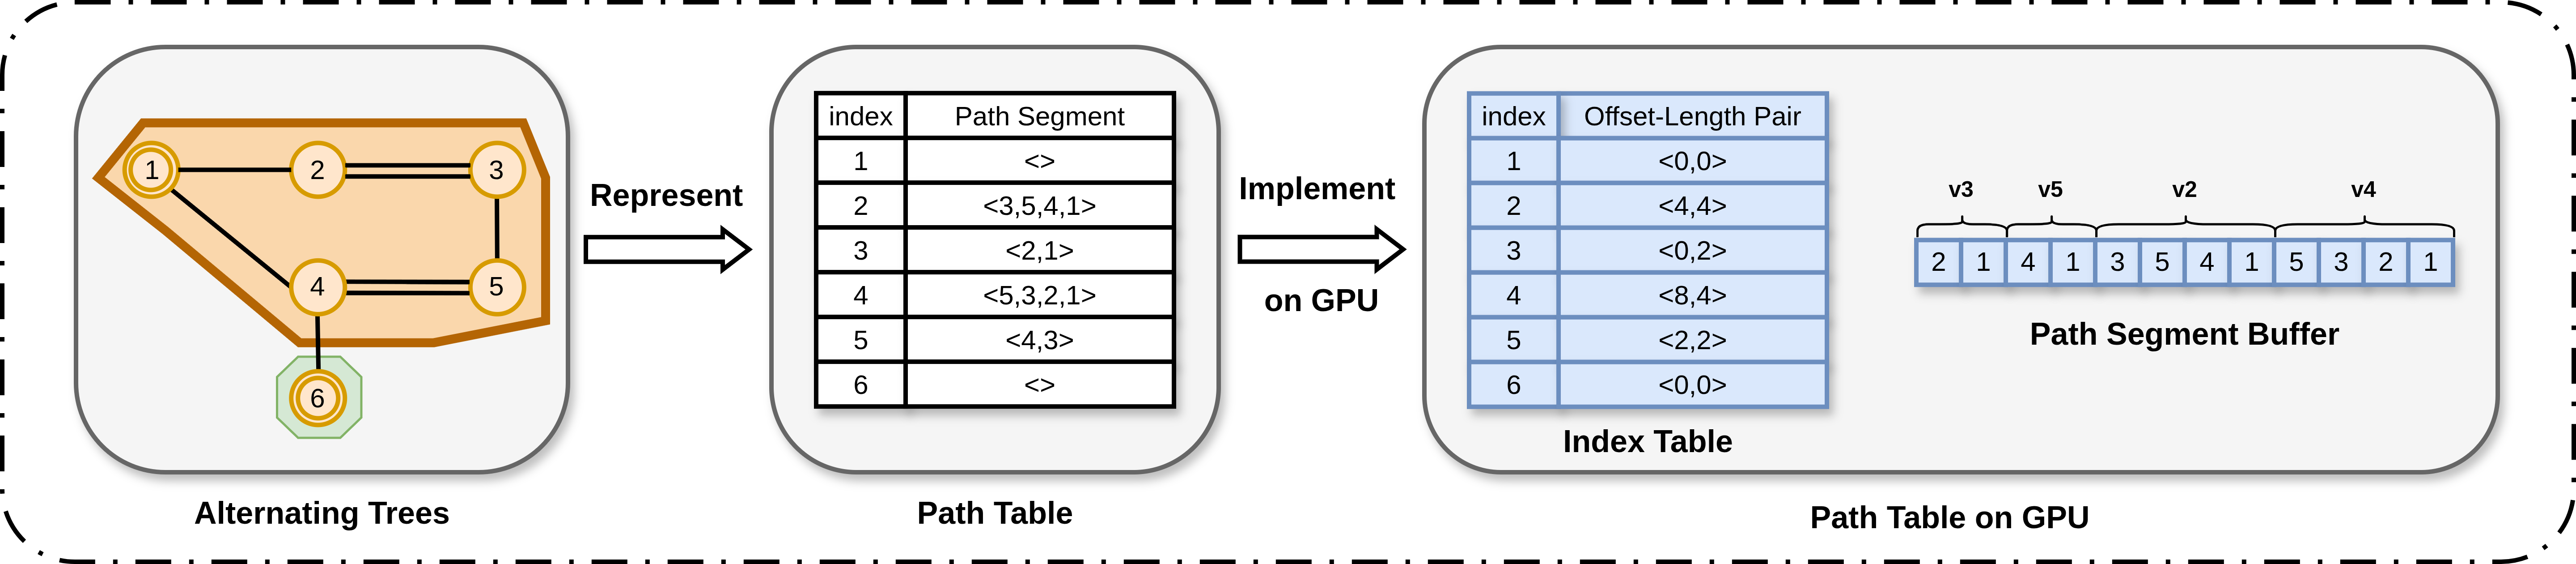
\includegraphics[width=1.0\columnwidth]{figures/diagrams/PathTableGPU.drawio.png}
	\captionsetup{skip=4pt}
	\caption{Alternating Trees, Path Table, and Path Table Implementation on GPUs}
	\label{Diagram:PathTable}
\vspace{-4pt}
\end{figure}

% Path Table on GPUs has an additional index table to be functional and efficient
A \emph{path table} compactly represents the alternating forest by mapping each even vertex to a \emph{path segment}.
As shown in Fig.~\ref{Diagram:PathTable}, roots such as 1 and 6 store empty segments.
Vertices added by expansion store the segment back to the previous even vertex: vertex~3 stores $\langle 2,1\rangle$, and vertex~5 stores $\langle 4,3\rangle$.
When blossom handling converts an odd vertex into an even vertex, it stores the segment through the blossom base; vertex~2 traces to base~1 through $3 \rightarrow 5 \rightarrow 4 \rightarrow 1$ and stores $\langle 3,5,4,1\rangle$.

On the GPU, the path table has an \emph{index table}, which maps each even vertex to an offset--length pair, and a contiguous \emph{path segment buffer}.
For example, vertex~2 stores $(4,4)$, meaning its four-element segment starts at offset~4.
% atomic counter
An atomic counter tracks the next available buffer offset.
Inserting a segment atomically reserves a contiguous region, writes the segment there, and records the offset--length pair in the index table.
% checking set
Similarly, the \emph{checking set} uses an array for newly added even vertices and an atomic counter for insertion positions.

\subsubsection{Two Workload Balancing Strategies}
\label{subsub:load-balancing}
Like other traversal algorithms, X-Blossom repeatedly processes incident edges of vertices in the current frontier across its three parallel phases.
Sparse graphs are stored in CSR format, where \emph{column indices} store neighbor vertices contiguously and \emph{row offsets} give each vertex's neighbor-list start.
Thus, processing frontier edges is equivalent to scanning the corresponding column-indices segments.
In Fig.~\ref{Diagram:Load-Balancing}, vertices 1--4 form the frontier; vertex~4 reads row-offset value 6 and scans $\langle v_3, v_5, v_6, v_7\rangle$.

% Two types of load-balancing strategy.
\begin{figure}[!h]
	\centering
	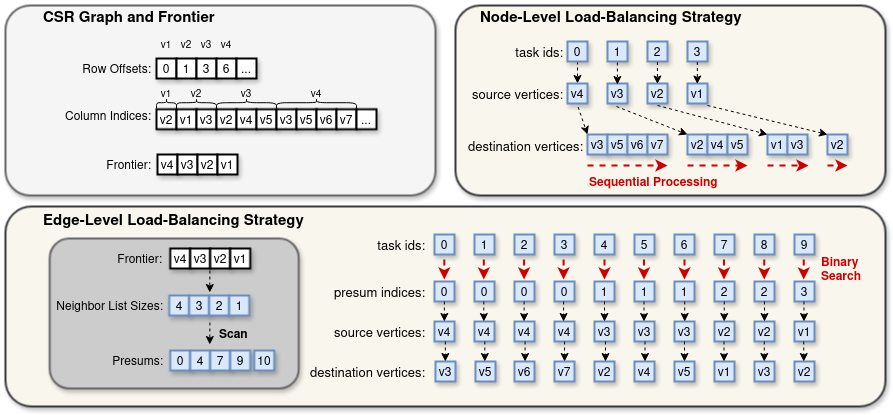
\includegraphics[width=1.0\columnwidth]{figures/diagrams/LoadBalanceStrategy.drawio.png}
	\captionsetup{skip=4pt}
	\caption{Two Load-Balancing Strategies}
	\label{Diagram:Load-Balancing}
\vspace{-4pt}
\end{figure}

% coarse-grained strategy
% In the coarse-grained, vertex-level strategy, each frontier vertex is treated as the indivisible unit of parallel work.
% Once an active frontier vertex is assigned to a thread, the thread loads the vertex’s neighbor-list offset and then serially scans and processes all of its incident edges.
Efficient frontier processing depends on workload distribution.
We consider two granularities: coarse-grained vertex-level (node-level) scheduling and fine-grained edge-level scheduling.
The vertex-level strategy creates one task per frontier vertex.
Each task reads \texttt{Row Offsets} and scans the corresponding \texttt{Column Indices} segment.
As Fig.~\ref{Diagram:Load-Balancing} shows, vertices 0--3 map to tasks 0--3, so different neighbor lists run in parallel but each list is scanned serially.
% Although the vertex-level strategy exposes parallelism across frontier vertices with minimal scheduling overhead, it underutilizes the available parallelism because all edges incident to a frontier vertex are independent and could, in principle, be processed concurrently. 
This design has low scheduling overhead but can underutilize parallelism because incident edges are independent.
It is also sensitive to skewed degree distributions: a high-degree frontier vertex can make its assigned thread process substantially more edges than other threads.
In the example, vertex $v_3$ has three neighbors while $v_1$ has one, so the thread processing $v_1$ can become idle while the thread processing $v_3$ remains busy.
% Moreover, in the context of X-Blossom, the imbalance is further amplified because a thread may also perform expensive blossom-related operations, such as detecting blossom bases and materializing blossoms, making the per-vertex workload even more irregular.
In X-Blossom, imbalance can be amplified when some vertices trigger costly blossom operations, such as tracing two endpoint-to-root paths to find the base and materializing the odd cycle.

% fine-grained strategy
The edge-level strategy instead creates one task per frontier edge.
It first builds an array of neighbor-list sizes and performs a prefix-sum scan, compacting sparse, skewed per-vertex work into dense per-edge tasks.
The resulting prefix-sum array records the cumulative number of incident edges contributed by frontier vertices, and its final entry gives the total number of frontier edges to process.
In Fig.~\ref{Diagram:Load-Balancing}, the frontier contributes ten edges, so ten tasks are generated.
Each task uses its ID to locate the corresponding frontier vertex by binary-searching the prefix-sum array.
For example, task IDs 4--6 map to prefix index~1, vertex $v_3$, and offsets 0--2, corresponding to neighbors $v_2$, $v_4$, and $v_5$.
By assigning one task per frontier edge, this strategy processes all incident edges in parallel rather than serially scanning each neighbor list.
However, compaction adds per-edge lookup overhead, which can be costly on platforms where binary searches and indirect indexing are expensive.
We evaluate both strategies in \S~\ref{subsubsec:exp_load_balancing}; edge-level load balancing is superior for X-Blossom++, whereas node-level scheduling is more effective for X-Blossom-Pro.

\begin{comment}
\subsection{On-the-fly Blossoeem-Base Identification}
The blossom-base identification is a prerequisite step before constructing a blossom as the concatenation of the paths from the base to each endpoint. 
This procedure takes as input an alternating tree, its root, and two even endpoints that form a blossom, and returns the blossom base. 
For example, given the alternating tree in Fig.~\ref{Diagram:OnTheFly} with root \(1\) and even endpoints \(9\) and \(11\), the goal of blossom-base identification is to return vertex \(5\) as the blossom base, which will later be used to construct the blossom cycle \(5 \to 6 \to 7 \to 8 \to 9 \to 11 \to 10 \to 5\).
% Path Table
During this process, each alternating tree is represented by a \emph{path table}, in which every even vertex stores the path segment from its preceding even vertex to itself (the right-hand table in Fig.~\ref{Diagram:OnTheFly}). For instance, even vertex \(9\) stores the segment \(\langle 9,8,7\rangle\). The root vertex \(1\) stores an empty path, since it has no preceding even vertex, and vertices \(2,4,6,8,10\) are odd, so they do not store any path segments in the table.


\begin{figure}[!h]
	\centering
	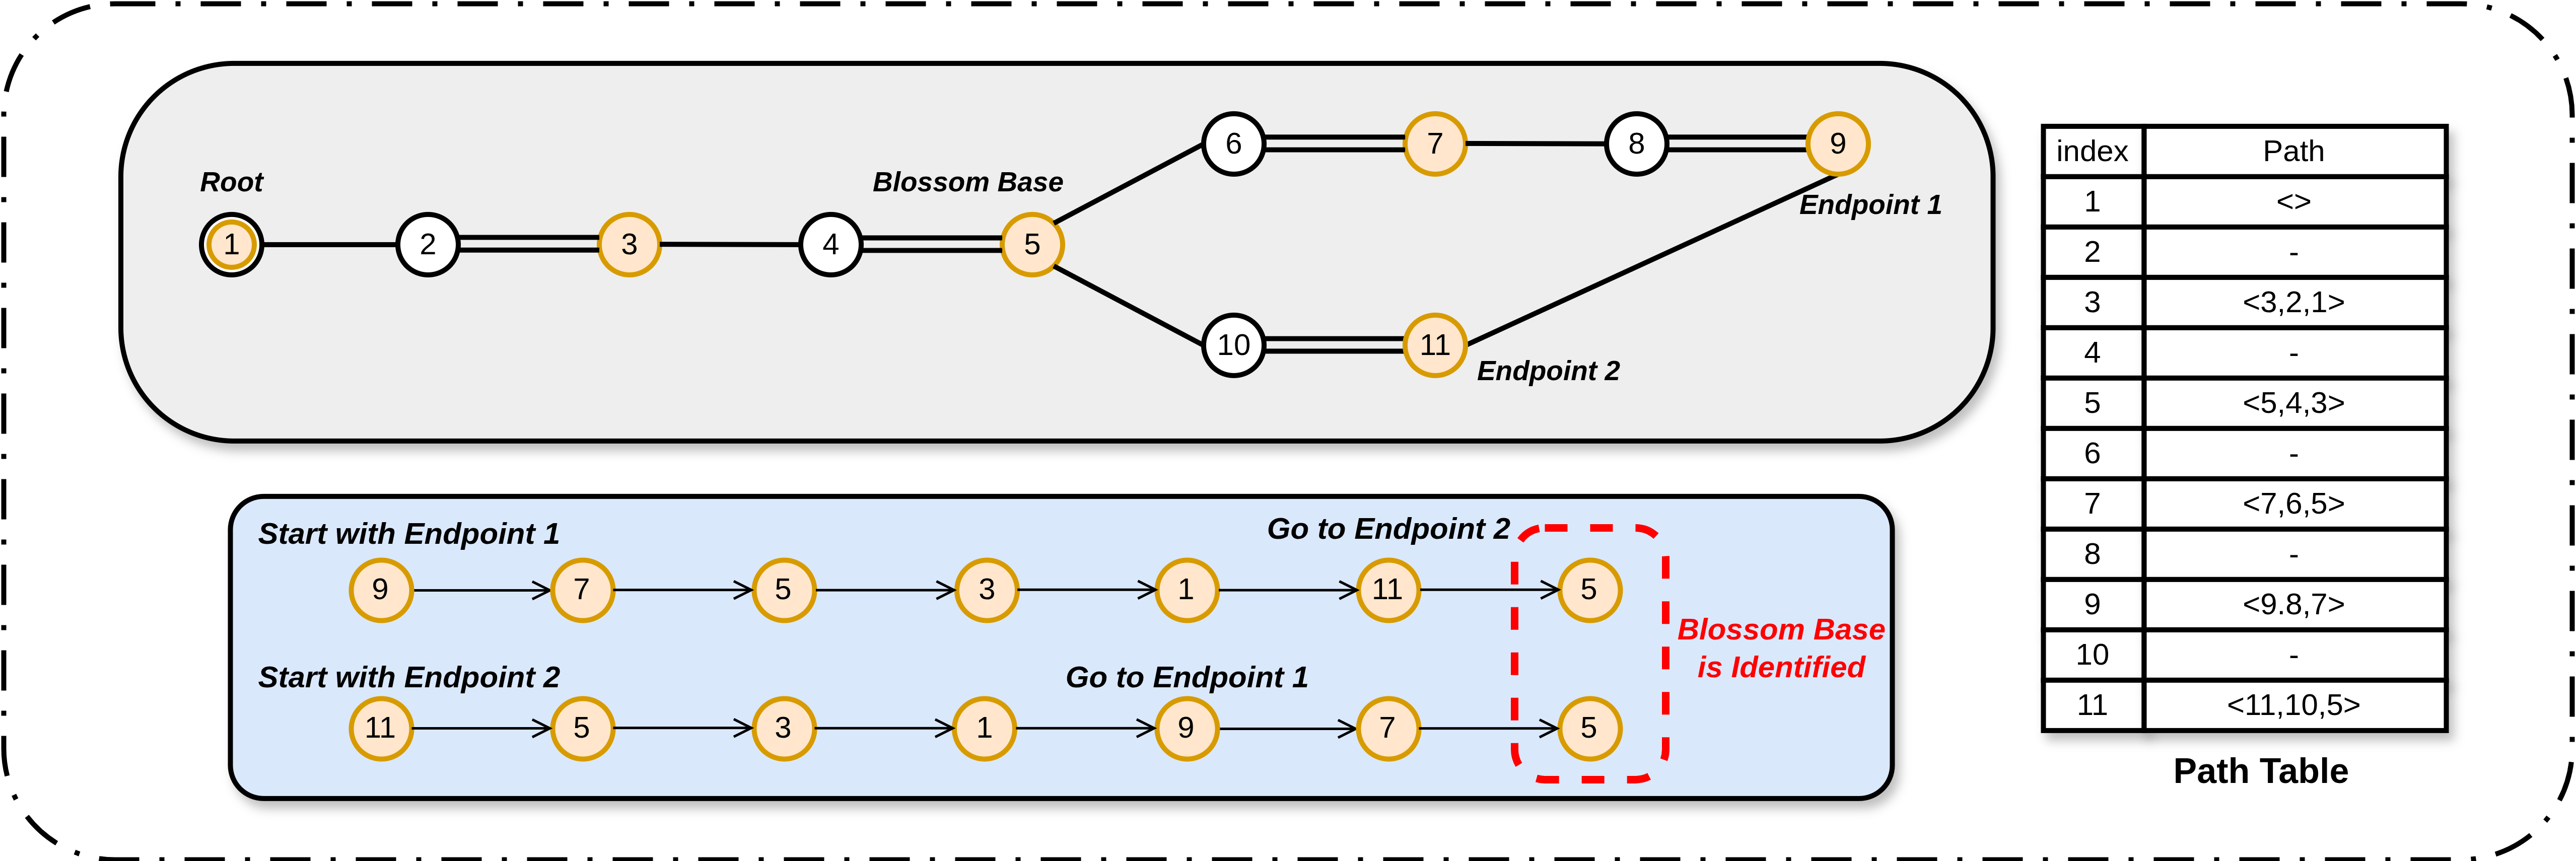
\includegraphics[width=1.0\columnwidth]{figures/diagrams/OnTheFlyIdenOnly.drawio.png}
	\captionsetup{skip=4pt}
	\caption{The On-The-Fly Blossom-Base Identification}
	\label{Diagram:OnTheFly}
\vspace{-4pt}
\end{figure}

The current blossom-base identification strategy reconstructs the full paths from each endpoint to the root and then identifies the base by locating the first divergence in these two paths. Concretely, starting from Endpoint~1 and Endpoint~2, it reconstructs the sequences
\(9 \to 8 \to 7 \to 6 \to 5 \to 4 \to 3 \to 2 \to 1\) and
\(11 \to 10 \to 5 \to 4 \to 3 \to 2 \to 1\),
stores them in temporary buffers, and scans the buffers from the root toward the leaves until the paths split at the outgoing edges \(5 \to 6\) and \(5 \to 10\). 
The last common vertex, \(5\), is then identified as the blossom base. 
This procedure is wasteful because it stores two full endpoint-to-root paths. In particular, the shared suffix from the base to the root,
\(5 \to 4 \to 3 \to 2 \to 1\), is materialized and scanned twice, once for each endpoint, even though this segment is not needed for constructing the blossom itself.

To avoid full endpoint-to-root path materialization, we adopt an \emph{on-the-fly} blossom-base identification scheme. 
We start two walks from the two endpoints simultaneously.
Each walk repeatedly moves from its current even vertex to its preceding even vertex until the two walks reach the same vertex. 
Whenever a walk reaches the root, it jumps to the opposite endpoint and continues. 
As illustrated in the lower panel of Fig.~\ref{Diagram:OnTheFly}, one walk follows \(9 \to 7 \to 5 \to 3 \to 1\) and then jumps to \(11 \to 5\), while the other walk follows \(11 \to 5 \to 3 \to 1\) and then jumps to \(9 \to 7 \to 5\). 
At the same iteration, both walks arrive at vertex \(5\), which is identified as the blossom base. 
% This base is subsequently used to materialize the blossom by combining the segments from the base to each endpoint.
    
\end{comment}
